\section{Diskussion}
\label{sec:Diskussion}

Die Untersuchung des Selektivverstärkers wurde durch den Sinusgenerator erschwert.
Die empfohlenen Einstellung aus der Versuchsanleitung konnten nicht am Sinusgenerator vorgenommen werden.
Bei jedem Versuch die Frequenz zu ändern, sprang der Sinusgenerator durch den ganzen Frequenzbereich.
Das Ablesen am AC-Millivoltmeter stellte sich genau so schwierig dar, da der Zeiger sich oft durch die ganze Skala frei bewegte.
Dadurch konnten weder klein- noch großschrittige Untersuchungen vorgenommen werden.
Es wurden Messpaare aufgenommen, die über einen kleinen Zeitraum stabil wirkten.
Teilweise wurden auch verschiedene Spannungen bei denselben Frequenzen notiert.
Eine Filterkurve ist nicht zu erkennen, somit sind Aussagen zum Selektivverstärker schwer zu treffen.
Der eigentliche Verlauf der Filterkurve ist in \autoref{fig:selektiv} zu sehen. 
Für die Gütebestimmung sollte ein klarer Peak und ein von dort in beide Richtungen ausgehender Fall zu erkennen sein.
Aus den aufgenommenen Messungen ist im Frequenzbereich 22.5 und 25.0 zwar eine Art Hoch zu erkennen.
Der Gesamtverlauf der aufgenommen Kurve fällt aber nur direkt nach diesem Hoch, ein Anstieg ist am Anfang des zu untersuchenden Frequenzintervalls kaum erkennbar.

\noindent
Die Stoffe $\ce{Dy2O3}$ und $\ce{Gd2O3}$ wurden verwendet, da die Messungen vor und nach dem Einführen der Probe sichtbare Differenzen haben.
Wie in der \autoref{tab:vergleich} zu sehen ist, wird der Theoriewert $\chi_T$ von dem im Experiment über die Widerstände ermittelten Wertes $\chi_R$ sehr gut angenähert.
Hierbei beträgt die Abweichung bei beiden Stoffe ca. 12-13\%.
Zwischen $\chi_T$ und $\chi_U$ besteht bei beiden Stoffen jeweils eine Abweichung von 66\%($\ce{Dy2O3}$)und 56\%($\ce{Gd2O3}$).
Das diese Abweichung höher liegt, war nach der Messung des Selektivverstärkers zu erwarten.
Die Spannung genau vom Gerät abzulesen war schwieriger als die Brückenschaltung minimal zu schalten.

\section{Anhang}
\label{sec:Anhang}
\begin{figure}
    \centering
    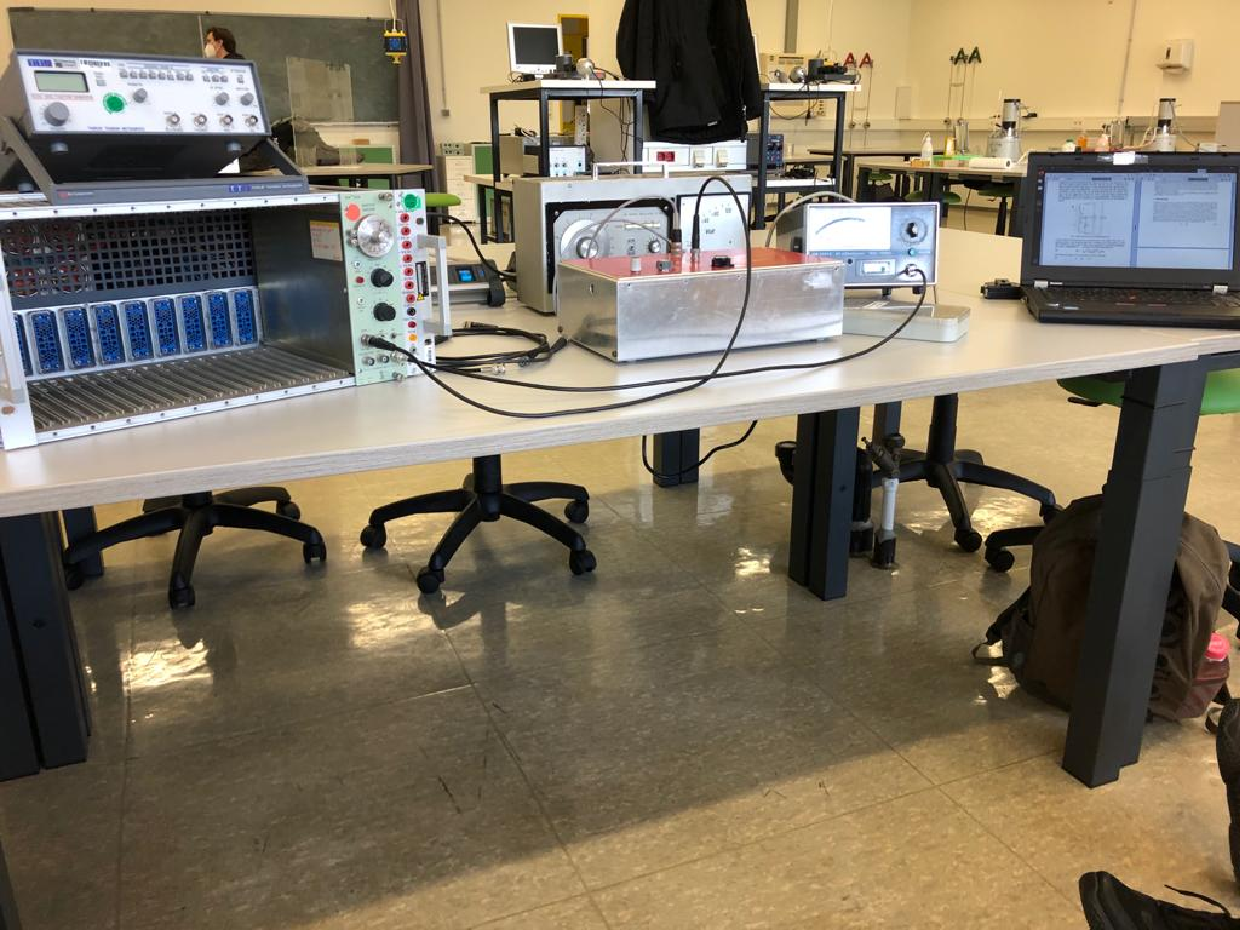
\includegraphics[width=\textwidth]{content/index.pdf}
    \caption{Das Foto vom Versuchsaufbau.Links im Bild ist der Selektivverstäarker unter einem Sinusgenerator zu sehen. 
    Die Box mit rotem Deckel ist die benutzte Brückenschaltung. 
    Hinter der Brückenschaltung ist der zweite Generator zu erkennen, welcher für die Messung der Suszeptibilität benutzt wurde.
    Rechts außen ist das AC-Millivoltmeter zu sehen.}
    \label{fig:datenselektiv1}
\end{figure}
\begin{figure}
    \centering
    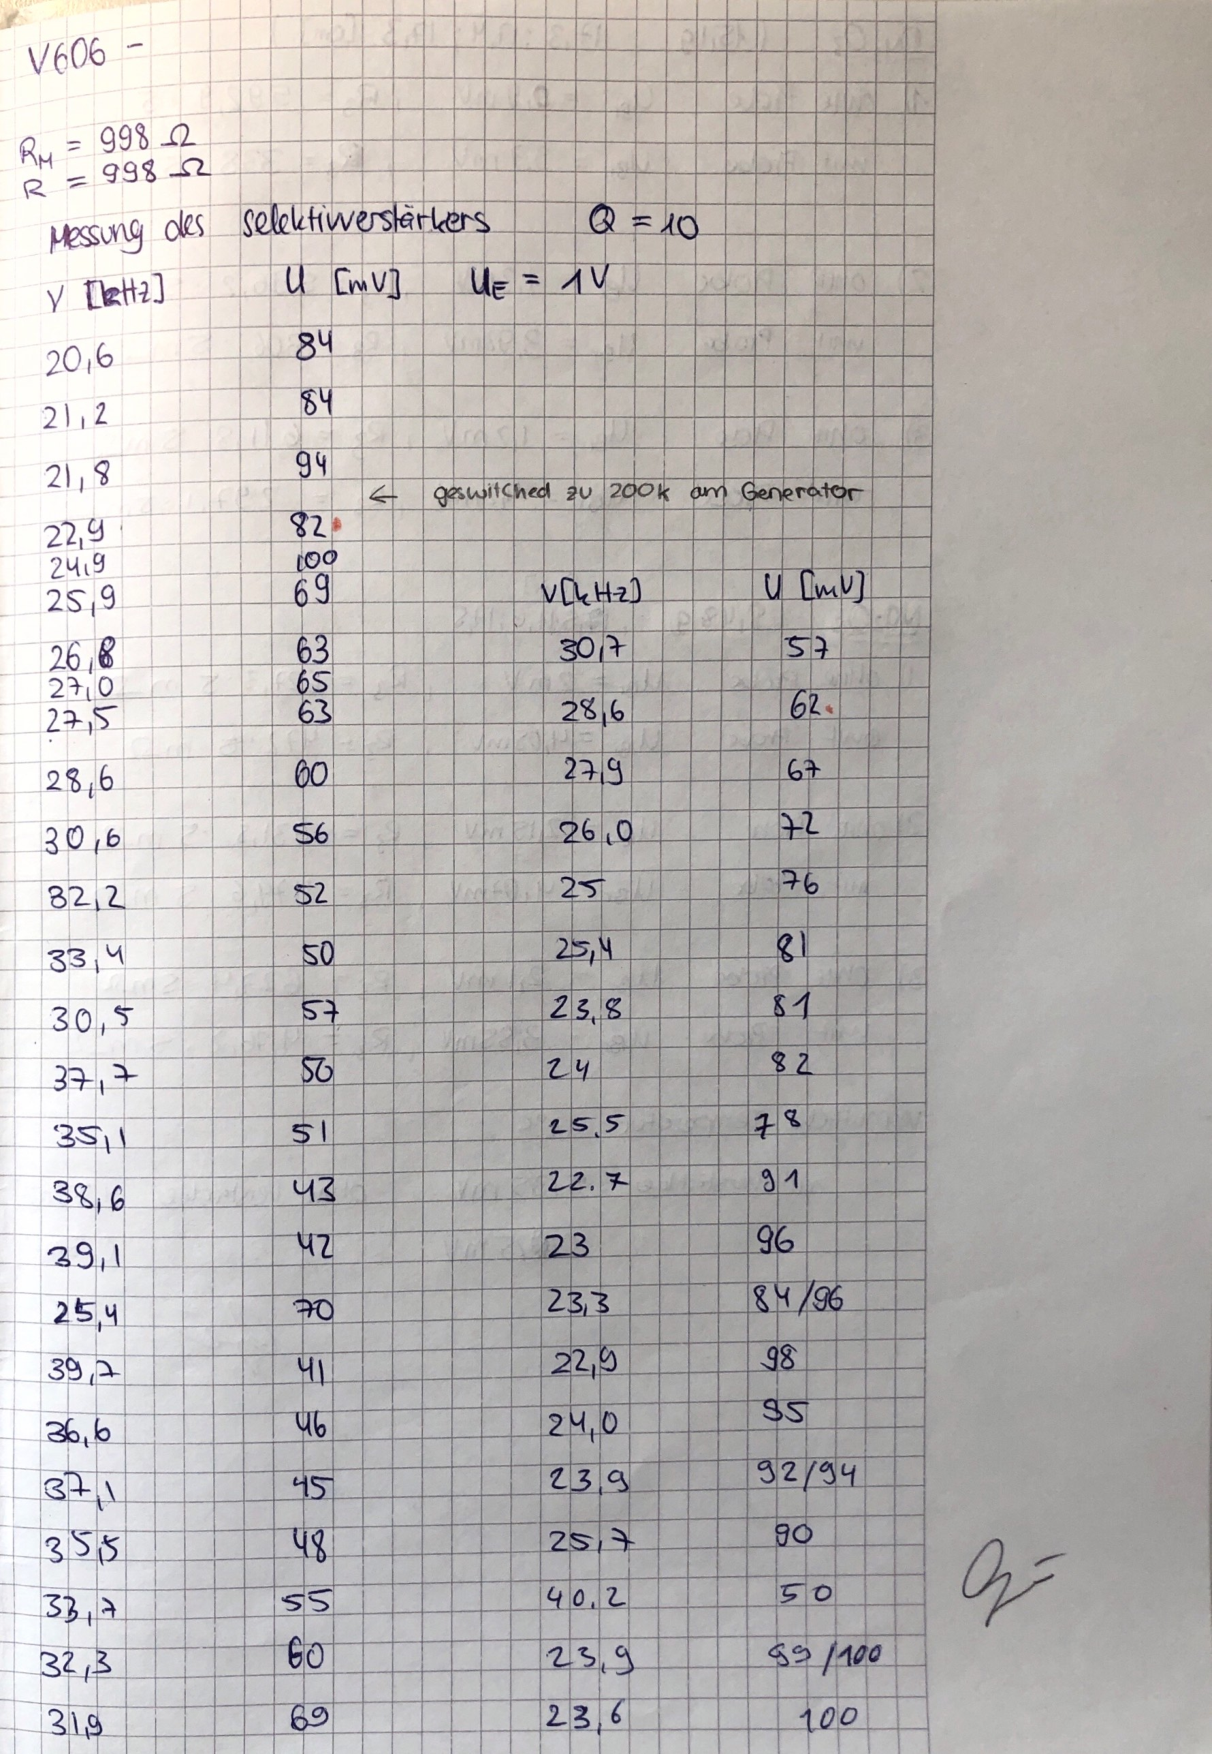
\includegraphics[width=\textwidth]{content/datenselektiv.pdf}
    \caption{Die aufgenommenen Werte für die Messung der Filterkurve des Selektivverstärkers.}
    \label{fig:datenselektiv2}
\end{figure}
\begin{figure}
    \centering
    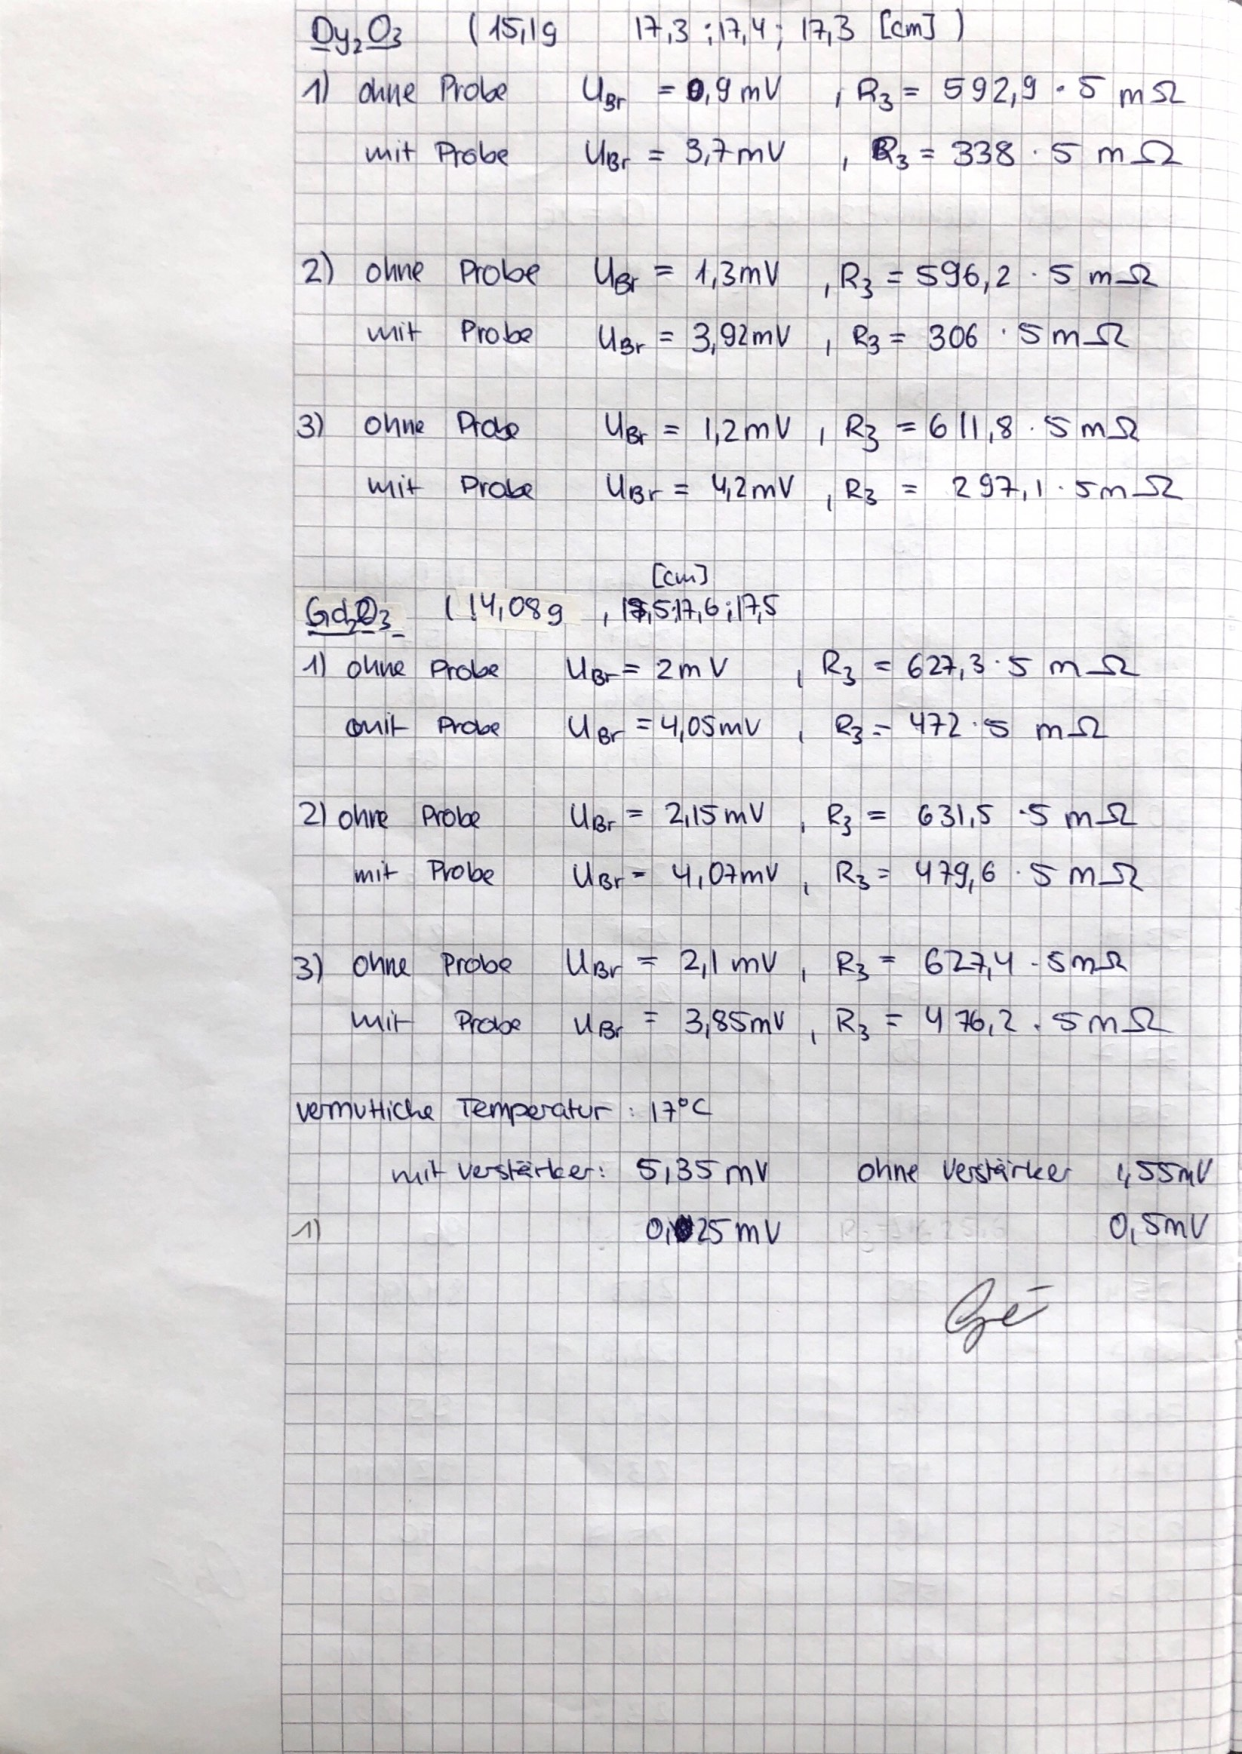
\includegraphics[width=\textwidth]{content/datenmessung.pdf}
    \caption{Die notierten Werte von der Vermessung der paramagnetischen Proben.}
    \label{fig:datenmessung}
\end{figure}
